\chapter{Forward proton analysis}
The forward proton detection system, described in Sec. 2.9, was installed to investigate the isospin dependence of the $^3$He($K^-,N$) reactions. In the current analysis, it was only used to evaluate the performance of the beam momentum reconstruction.

The analysis method was basically same as the neutron case(see Sec. 3.5), except that we should consider bended trajectories in flight-length calculations, and we should identify the particle species such as pions, protons and deuterons. Although the CVC can be also used for the same purpose to extend the acceptance for high momentum particles ($>$1 GeV/$c$), it was not included in the current analysis.
%Momenta of the forward charged particles were measured with the time-of-flight method, while bending angles at the Ushiwaka magnet were used for the particle identification only.
\section{Trajectory reconstruction}
The trajectory of a forward charged particle was determined with measured three points. They were the reaction vertex and positions at the FDC1 and at the PC. The reaction vertex was determined with the beam trajectory and the CDC track(s). The position at FDC1 was obtained from the track in the FDC1. The $x$ and $z$ positions at the PC was defined by a central position of the fired segments and $y$ position by the timing difference of the signals from two PMTs at both ends of the counter. The former two positions were used to defined out-going direction from the reaction point and an arc was employed as the trajectory in the dipole field of the Ushiwaka to smoothly change the direction toward the hit position at the PC. We assumed an uniform field in the Ushiwaka magnet and an effective field length of $96$ cm was, as a result of a simulation study with a realistic magnetic-field calculation using TOSCA. With this simple description of the particle trajectory, an estimation of the flight length was found to be accurate within a 1 mm level. 

\section{Particle identification}
Once we obtained the flight length of the particle, the velocity of the particle ($\beta$) was calculated as described in Sec. 3.5.1. Then, the mass squared of the particle was calculated with a bending radius at the Ushiwaka, $\rho_{\rm Ushiwaka}$, which was also obtained in the trajectory reconstruction. The mass squared was calculated as
\begin{eqnarray*}
M^2 &=& \left(\frac{cB_{\rm Ushiwaka}}{\rho_{\rm Ushiwaka}}\right)^2\times\frac{1-\beta^2}{\beta^2},
\end{eqnarray*}
where $B_{\rm Ushiwaka}$ is the field strength of the Ushiwaka magnet. Figure \ref{fig-pcpid} shows a distribution of mass squared, where pions, protons and deuterons were successfully identified. Note that the field strength of the Ushiwaka used in the calculation was tuned to adjust the peak position corresponds to protons.
\begin{figure}[]
\begin{center}
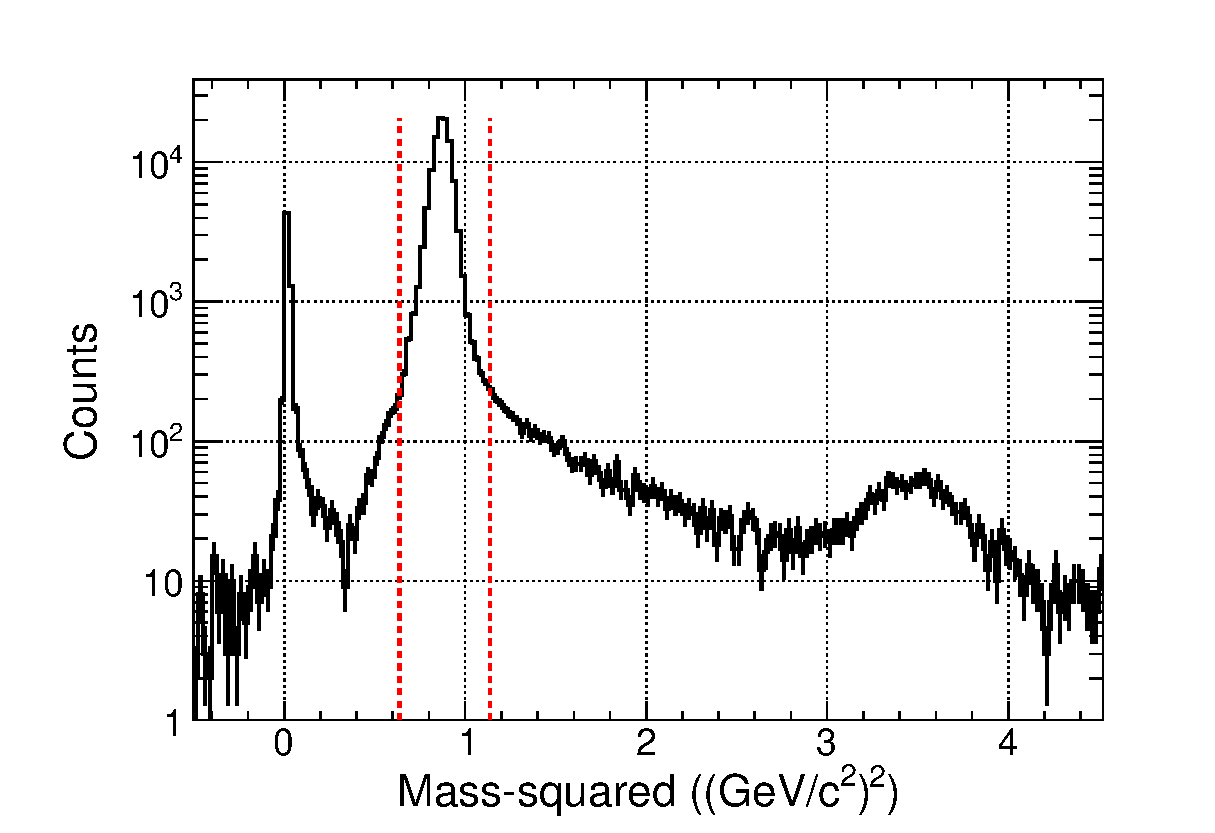
\includegraphics[width=10cm]{./fig/pc-pid.eps}
\caption[Particle identification with the forward charged particle spectrometer.]{Particle identification with the forward charged particle spectrometer. The two dotted lines show the selection region for protons. Pion and deuteron peaks are also seen.}
\label{fig-pcpid}
\end{center}
\end{figure}  


\section{Momentum reconstruction}
The momentum resolution with the bending angle at the Ushiwaka was limited to $\sim$20 MeV/$c$ at 1 GeV/$c$. Therefore the bending angle was used only for the particle identification. The momentum was recalculated with TOF information by using Eq. (3.4). Here, we considered velocity changes by energy losses not only for the kaon beam but also for forward charged particles. The momentum was iteratively searched to give the measured TOF.

\section{Calibration and Momentum scale}
The relative timing offsets among the segments in the PC were adjusted with the pion beam data. The reconstructed beam momentum was used to calculate the standard of the TOF between T0 and the PC, and the time offset was tuned to adjust a measured TOF to it. The time-walk effect was also corrected at the same time. A typical TOF resolution was 180 ps ($\sigma$) for pions. Note that a proton deposit larger energy on the scintillator, resulting in a better TOF resolution.

We reconstructed the $\pi p$ and $K^-p$ invariant mass distributions in the production data to see the expected peaks of the $\Lambda$ and $\Lambda(1520)$, respectively. These peaks were successfully observed as shown in Fig. \ref{fig-pcpeaks}. The peak positions were consistent with the PDG masses within $\sim$1 MeV/$c$, which indicated the good accuracy of the momentum scale for the forward charged particles.

\begin{figure}[]
\begin{center}
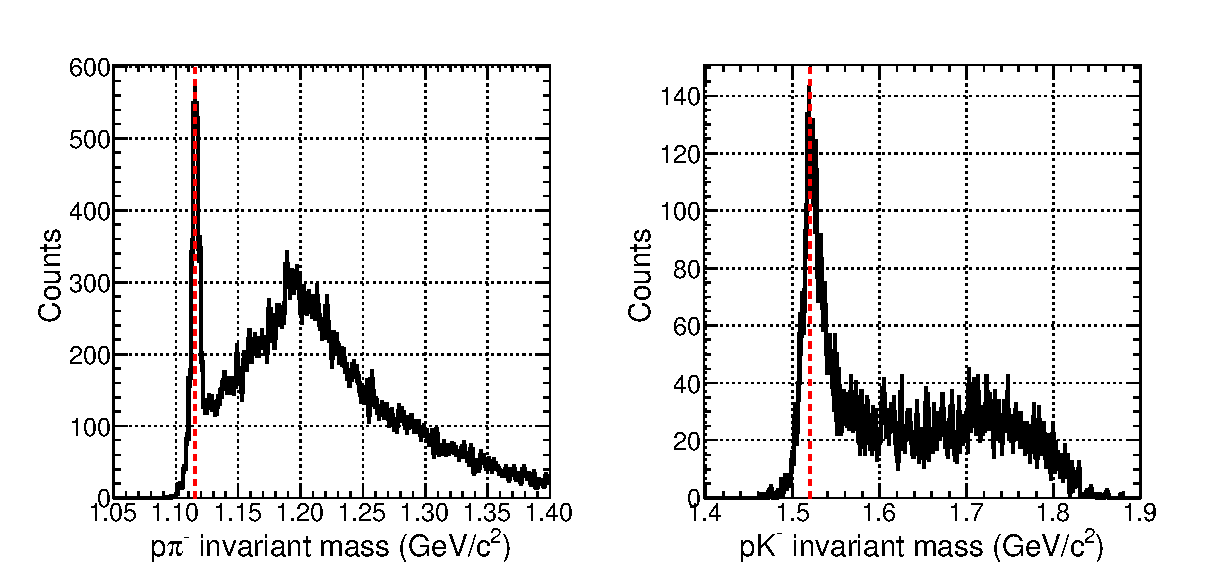
\includegraphics[width=\columnwidth]{./fig/pc-peaks.eps}
\caption[Invariant mass distributions of $p\pi^-$ and $pK^-$]{Invariant mass distributions of (left) $p\pi^-$ and (right) $pK^-$, where $\Lambda$ and $\Lambda(1520)$ were clearly identified, respectively. The protons were detected with the PC and the pions and kaons were detected with the CDS. The red dotted lines indicate the masses of $\Lambda$ and $\Lambda(1520)$ in the PDG.}
\label{fig-pcpeaks}
\end{center}
\end{figure}  

\section{Beam-though run}
The forward charged particle detection system was used as a reference of the beam momentum measurement. We took dedicated data of $\pi^+$ and proton beams, which transported through the beam spectrometer and the Ushiwaka to the PC. The field strength of the Ushiwaka was fixed to be the same value with the production runs. The $\pi^+$ data was used to calibrate the relative timing offset of the PC segments, and then we compared two momentum measurements of proton beams, i.e., with the beam spectrometer and with the forward charged particle detection system. In the analysis of forward spectrometer, we defined the vertex point by the extrapolation of the BPC track at the FF.

The result of the beam momentum evaluation is given in Sec. 3.3.4.